\chapter{Prioridade de Requisitos com Use Case Points}\label{cap:9-prio-req}

A priorização de requisitos é uma etapa fundamental para alinhar o desenvolvimento do sistema às necessidades dos stakeholders e otimizar o uso de recursos. Segundo a abordagem apresentada em aula, a classificação dos requisitos pode ser feita em três níveis: Essencial (crítico), Importante e Desejável (útil). A priorização facilita o diálogo entre usuários e equipe de desenvolvimento, permitindo identificar o conjunto mínimo de funcionalidades necessárias para atender aos objetivos do projeto.

Neste capítulo, será realizada uma análise de redução de escopo baseada na técnica de Use Case Points (UCP) calculada no capítulo anterior, visando uma diminuição de pelo menos 30\% no custo estimado do projeto. Para isso, serão removidos, primeiramente, os casos de uso de menor prioridade (desejáveis), seguidos dos importantes, até atingir a meta de redução.

\section{Redução de 30\% no Custo do Projeto}

O valor total estimado para o projeto, conforme o cálculo dos Use Case Points no capítulo 8, foi de:

\begin{itemize}
    \item \textbf{UCP total:} 52
    \item \textbf{Horas estimadas:} 520
\end{itemize}

Reduzindo em 30\%:

\begin{itemize}
    \item \textbf{UCP reduzido:} 52 $\times$ 0,7 = \textbf{36,4}
    \item \textbf{Horas reduzidas:} 520 $\times$ 0,7 = \textbf{364}
\end{itemize}

Sabendo que o UCP deve ser reduzido para, pelo menos, $36,4$, o próximo passo é identificar quais casos de uso podem ser removidos para atingir essa meta. Portanto, trabalharemos com a redução do valor do UUCP que, de acordo com o capítulo \ref{cap:8-ger-req-use-case-points} é de 93. Neste caso, abaixo consta o cálculo que demonstra a redução necessária:

Cálculo do valor mínimo de UUCP para atingir pelo menos $UCP = 36,4$:
\begin{align*}
    UUCP \times TCF \times ECF &= UCP\\
    UUCP &= \frac{UCP}{TCF \times ECF}\\
    &= \frac{36,4}{1,055 \times 0,53}\\
    &= 65,1
\end{align*}

Portanto, o valor mínimo de UUCP necessário para atingir a meta de redução é de 65,1. Considerando que o UUCP original é 93, a redução necessária é:
\begin{align*}
    UUCP_{Reduzir} &= UUCP - UUCP_{min}\\
    &= 93 - 65,1\\
    &= 27,9
\end{align*}

\section{Seleção dos Casos de Uso Necessários e Suficientes}

Para atingir a meta de redução de pelo menos 30\% no custo do projeto, é necessário que o valor do UUCP (soma dos pontos dos atores e dos casos de uso) seja inferior a 65,1, conforme demonstrado anteriormente. O UUCP original do sistema é 93, composto por UAW = 8 (atores) e UUCW = 85 (casos de uso). Assim, a redução mínima necessária é de 27,9 pontos no UUCP, o que implica a remoção de casos de uso de menor prioridade até que o novo UUCP seja igual ou inferior a 65,1.

A estratégia adotada consiste em remover, primeiramente, os casos de uso classificados como desejáveis, seguidos dos importantes de menor impacto, sempre preservando as funcionalidades essenciais para o funcionamento do sistema.

\subsection{Classificação dos Casos de Uso por Prioridade}

Com base nos requisitos funcionais refinados (capítulo 6), a classificação dos casos de uso é:

\begin{itemize}
    \item \textbf{Essenciais:} RF01 (Cadastro de usuário), RF03 (Registro de refeições), RF04 (Consulta nutricional via LLM), RF05 (Armazenamento de dados nutricionais)
    \item \textbf{Importantes:} RF02 (Autenticação), RF06 (Dashboard), RF08 (Chat LLM), RF10 (Edição/exclusão de refeições)
    \item \textbf{Desejáveis:} RF07 (Filtros temporais), RF09 (Exportação de relatórios)
\end{itemize}

\subsection{Remoção dos Casos de Uso de Menor Prioridade}

A distribuição dos pontos dos casos de uso (UUCW) é:

\begin{itemize}
    \item \textbf{Simples (5 pontos):} RF01, RF02, RF07, RF09, RF10
    \item \textbf{Médio (10 pontos):} RF03, RF05, RF08
    \item \textbf{Complexo (15 pontos):} RF04, RF06
\end{itemize}

O UAW permanece constante em 8, pois não há alteração nos atores do sistema. Portanto, a redução será realizada exclusivamente sobre o UUCW.

% Remoção dos casos de uso de menor prioridade
Removendo inicialmente os casos de uso desejáveis (RF07 e RF09):

\begin{itemize}
    \item Pontos removidos: 5 (RF07) + 5 (RF09) + 1 (ator simples do serviço de exportação de relatórios) = 11
    \item UUCW restante: 85 - 10 = 75
    \item UAW restante: 8 - 1 = 7
    \item UUCP restante: 7 + 75 = 82
\end{itemize}

Ainda não atingiu a meta. Removendo o caso de uso importante de menor impacto (RF10):

\begin{itemize}
    \item Pontos removidos: 5 (RF10)
    \item UUCW restante: 75 - 5 = 70
    \item UUCP restante: 7 + 70 = 77
\end{itemize}

Ainda não atingiu a meta. Removendo o próximo importante (RF08):

\begin{itemize}
    \item Pontos removidos: 10 (RF08)
    \item UUCW restante: 70 - 10 = 60
    \item UUCP restante: 7 + 60 = 67
\end{itemize}

Ainda não atingiu a meta. Removendo o requisito de autenticação do usuário (RF02), que também possui um ator de serviço externo (2 pontos):

\begin{itemize}
    \item Pontos removidos: 5 (RF02) + 2 (ator médio do serviço externo de autenticação) = 7
    \item UUCW restante: 60 - 5 = 55
    \item UAW restante: 7 - 2 = 5
    \item UUCP restante: 5 + 55 = 60
\end{itemize}

Neste ponto, o UUCP total é 60, o que representa uma redução de 33 pontos em relação ao original (93 - 60 = 33), superando a meta de redução estabelecida.

\textbf{Resumo dos Casos de Uso Mantidos:}

\begin{itemize}
    \item RF01: Cadastro de usuário (5 pontos)
    \item RF03: Registro de refeições (10 pontos)
    \item RF04: Consulta automática de dados nutricionais via LLM (15 pontos)
    \item RF05: Armazenamento de dados nutricionais (10 pontos)
    \item RF06: Dashboard com gráficos de consumo (15 pontos)
\end{itemize}

\textbf{Total UUCW mantido:} 5 + 10 + 15 + 10 + 15 = 55

\textbf{UUCP final:} 5 (UAW) + 55 (UUCW) = 60

\textbf{Redução de UUCP final:} (93 - 60) / 93 = 35,5\%

A redução obtida supera a meta estabelecida, mantendo o equilíbrio entre otimização de custos e atendimento aos objetivos do projeto.

\textbf{Atores Remanescentes:} Após a redução de escopo, permanecem os seguintes atores no sistema: usuário final via interface web (ator complexo), serviço externo de autenticação (removido junto com RF02), e demais serviços associados aos casos de uso mantidos. O UAW final é 5, compatível com os casos de uso remanescentes.

\section{Listagem dos Casos de Uso Após Redução}

\begin{longtable}{|l|l|l|}
\caption{Casos de Uso mantidos após redução de $35,5$\% no custo}
\label{tab:casos-uso-reducao}\\
\hline
\textbf{Código} & \textbf{Descrição} & \textbf{Prioridade} \\
\hline
\endfirsthead
\endhead
RF01 & Cadastro de usuário & Essencial \\
\hline
RF03 & Registro de refeições & Essencial \\
\hline
RF04 & Consulta automática de dados nutricionais via LLM & Essencial \\
\hline
RF05 & Armazenamento de dados nutricionais & Essencial \\
\hline
RF06 & Dashboard com gráficos de consumo & Importante \\
\hline
\end{longtable}

\noindent Os casos de uso removidos (RF07, RF08, RF09, RF10) correspondem às funcionalidades de filtros temporais, chat com o LLM, exportação de relatórios e edição/exclusão de refeições, consideradas de menor prioridade para o funcionamento mínimo do sistema.

O diagrama de casos de uso atualizado, refletindo a redução de escopo, é apresentado na Figura \ref{fig:casos-uso-reducao}.
\begin{figure}[h]
    \centering
    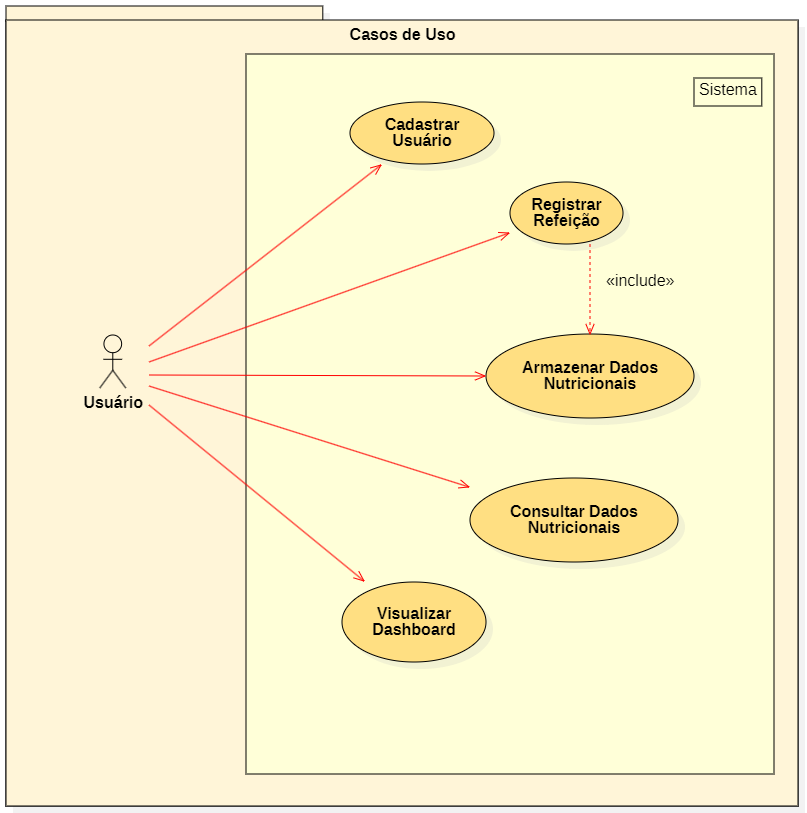
\includegraphics[width=0.8\textwidth]{Figuras/casos-uso-reducao.png}
    \caption{Diagrama de Casos de Uso após redução de escopo}
    \label{fig:casos-uso-reducao}
\end{figure}

\section{Cálculo do Novo Valor de Use Case Points (UCP) após Redução}

Considerando o novo valor de UUCP = 60, e mantendo os fatores técnicos (TCF) e ambientais (ECF) já calculados no Capítulo \ref{cap:8-ger-req-use-case-points}, temos:

\begin{itemize}
    \item \textbf{UUCP:} 60
    \item \textbf{TCF:} 1,055
    \item \textbf{ECF:} 0,53
\end{itemize}

O cálculo do novo valor de UCP é:

\begin{align*}
    UCP &= UUCP \times TCF \times ECF \\
    &= 60 \times 1,055 \times 0,53 \\
    &= 63,3 \times 0,53 \\
    &= 33,549 \\
    &\approx \textbf{33,5}
\end{align*}

Portanto, o novo valor de UCP após a redução de escopo é \textbf{33,5}. Considerando a estimativa de 10 horas por UCP:

\begin{itemize}
    \item \textbf{Horas estimadas:} $33,5 \times 10 = 335$
\end{itemize}

Esse resultado demonstra que a redução de escopo atingiu e superou a meta de redução de pelo menos 30\% no custo do projeto.

\section{Considerações Finais}

A priorização e redução de requisitos são etapas críticas para garantir que o sistema atenda às necessidades essenciais dos usuários, mantendo a viabilidade do projeto. A técnica de Use Case Points permitiu uma análise objetiva do custo e da complexidade dos casos de uso, facilitando a tomada de decisão sobre quais funcionalidades manter no escopo inicial.

A redução de 30\% no custo foi alcançada com a remoção de casos de uso desejáveis e importantes, preservando as funcionalidades essenciais para o funcionamento do sistema. Essa abordagem garante que o projeto possa ser implementado de forma eficiente, com foco nas necessidades mais críticas dos usuários.